The Pozyx Creator Kit comes with anchors and several tags. Anchors are mounted 
on the walls and are used to position the tags. Multiple tags may be positioned
at the same time.
The Pozyx Creator kit uses ultrawideband (UWB) signals with the two-way ranging protocol to localize the tag. 
The tag is mounted on custom 3D printed wearables which the participant can wear as 
a wrist-watch or a necklace. Through trial-and-error and consultation with the Pozyx Creator Documentation
\cite{noauthor_hardware_nodate,noauthor_configuration_nodate}
it was determined that the accuracy of the system depends on factors listed below:

\begin{itemize}
    \item Number of anchors
    \item Position of anchors
\end{itemize}

These variables were modified to achieve satisfactory actual position error
and standard deviation below the expected error of 30 cm for UWB systems. The 
protocol for obtaining data and evaluating the actual position error and 
standard deviation will be described.

% ----------------------------------------------------------------------------------------------------
\section{Methodology}
This protocol tests the X, Y, and Z positional accuracy of the Pozyx Creator system in the Independent
Living Suite (ILS) at the Glenrose Rehabilitation Hospital by having a participant stand at 
a specific location in each room. Permanent appliances or furniture such as the stove
or dining table were used as much as possible to ensure that the experiment is repeatable.

\subsection{Setup}
Masking tape was used to mark the locations where the participant should place their feet.
The following procedure was followed to place the tape:
\begin{enumerate}
    \item Using a measuring tape, measure 1 meter out from the middle of the 
    appliance or furniture and place a 20 cm piece of tape centered on, perpendicular to
    and underneath the measuring tape (the tips of the participant's toes should be 1 meter
    away from the appliance).\label{step1}
    \item Place parallel tape on the sides of the tape placed in Step \ref{step1} to constrain
    the feet to a box. (The participant should have their toes on the tape perpendicular to the
    measuring tape and usually facing the appliance or furniture).
    Figure \ref{fig:tape} outlines some examples of tape placements.
\end{enumerate}


\begin{figure}[ht]
    \centering
    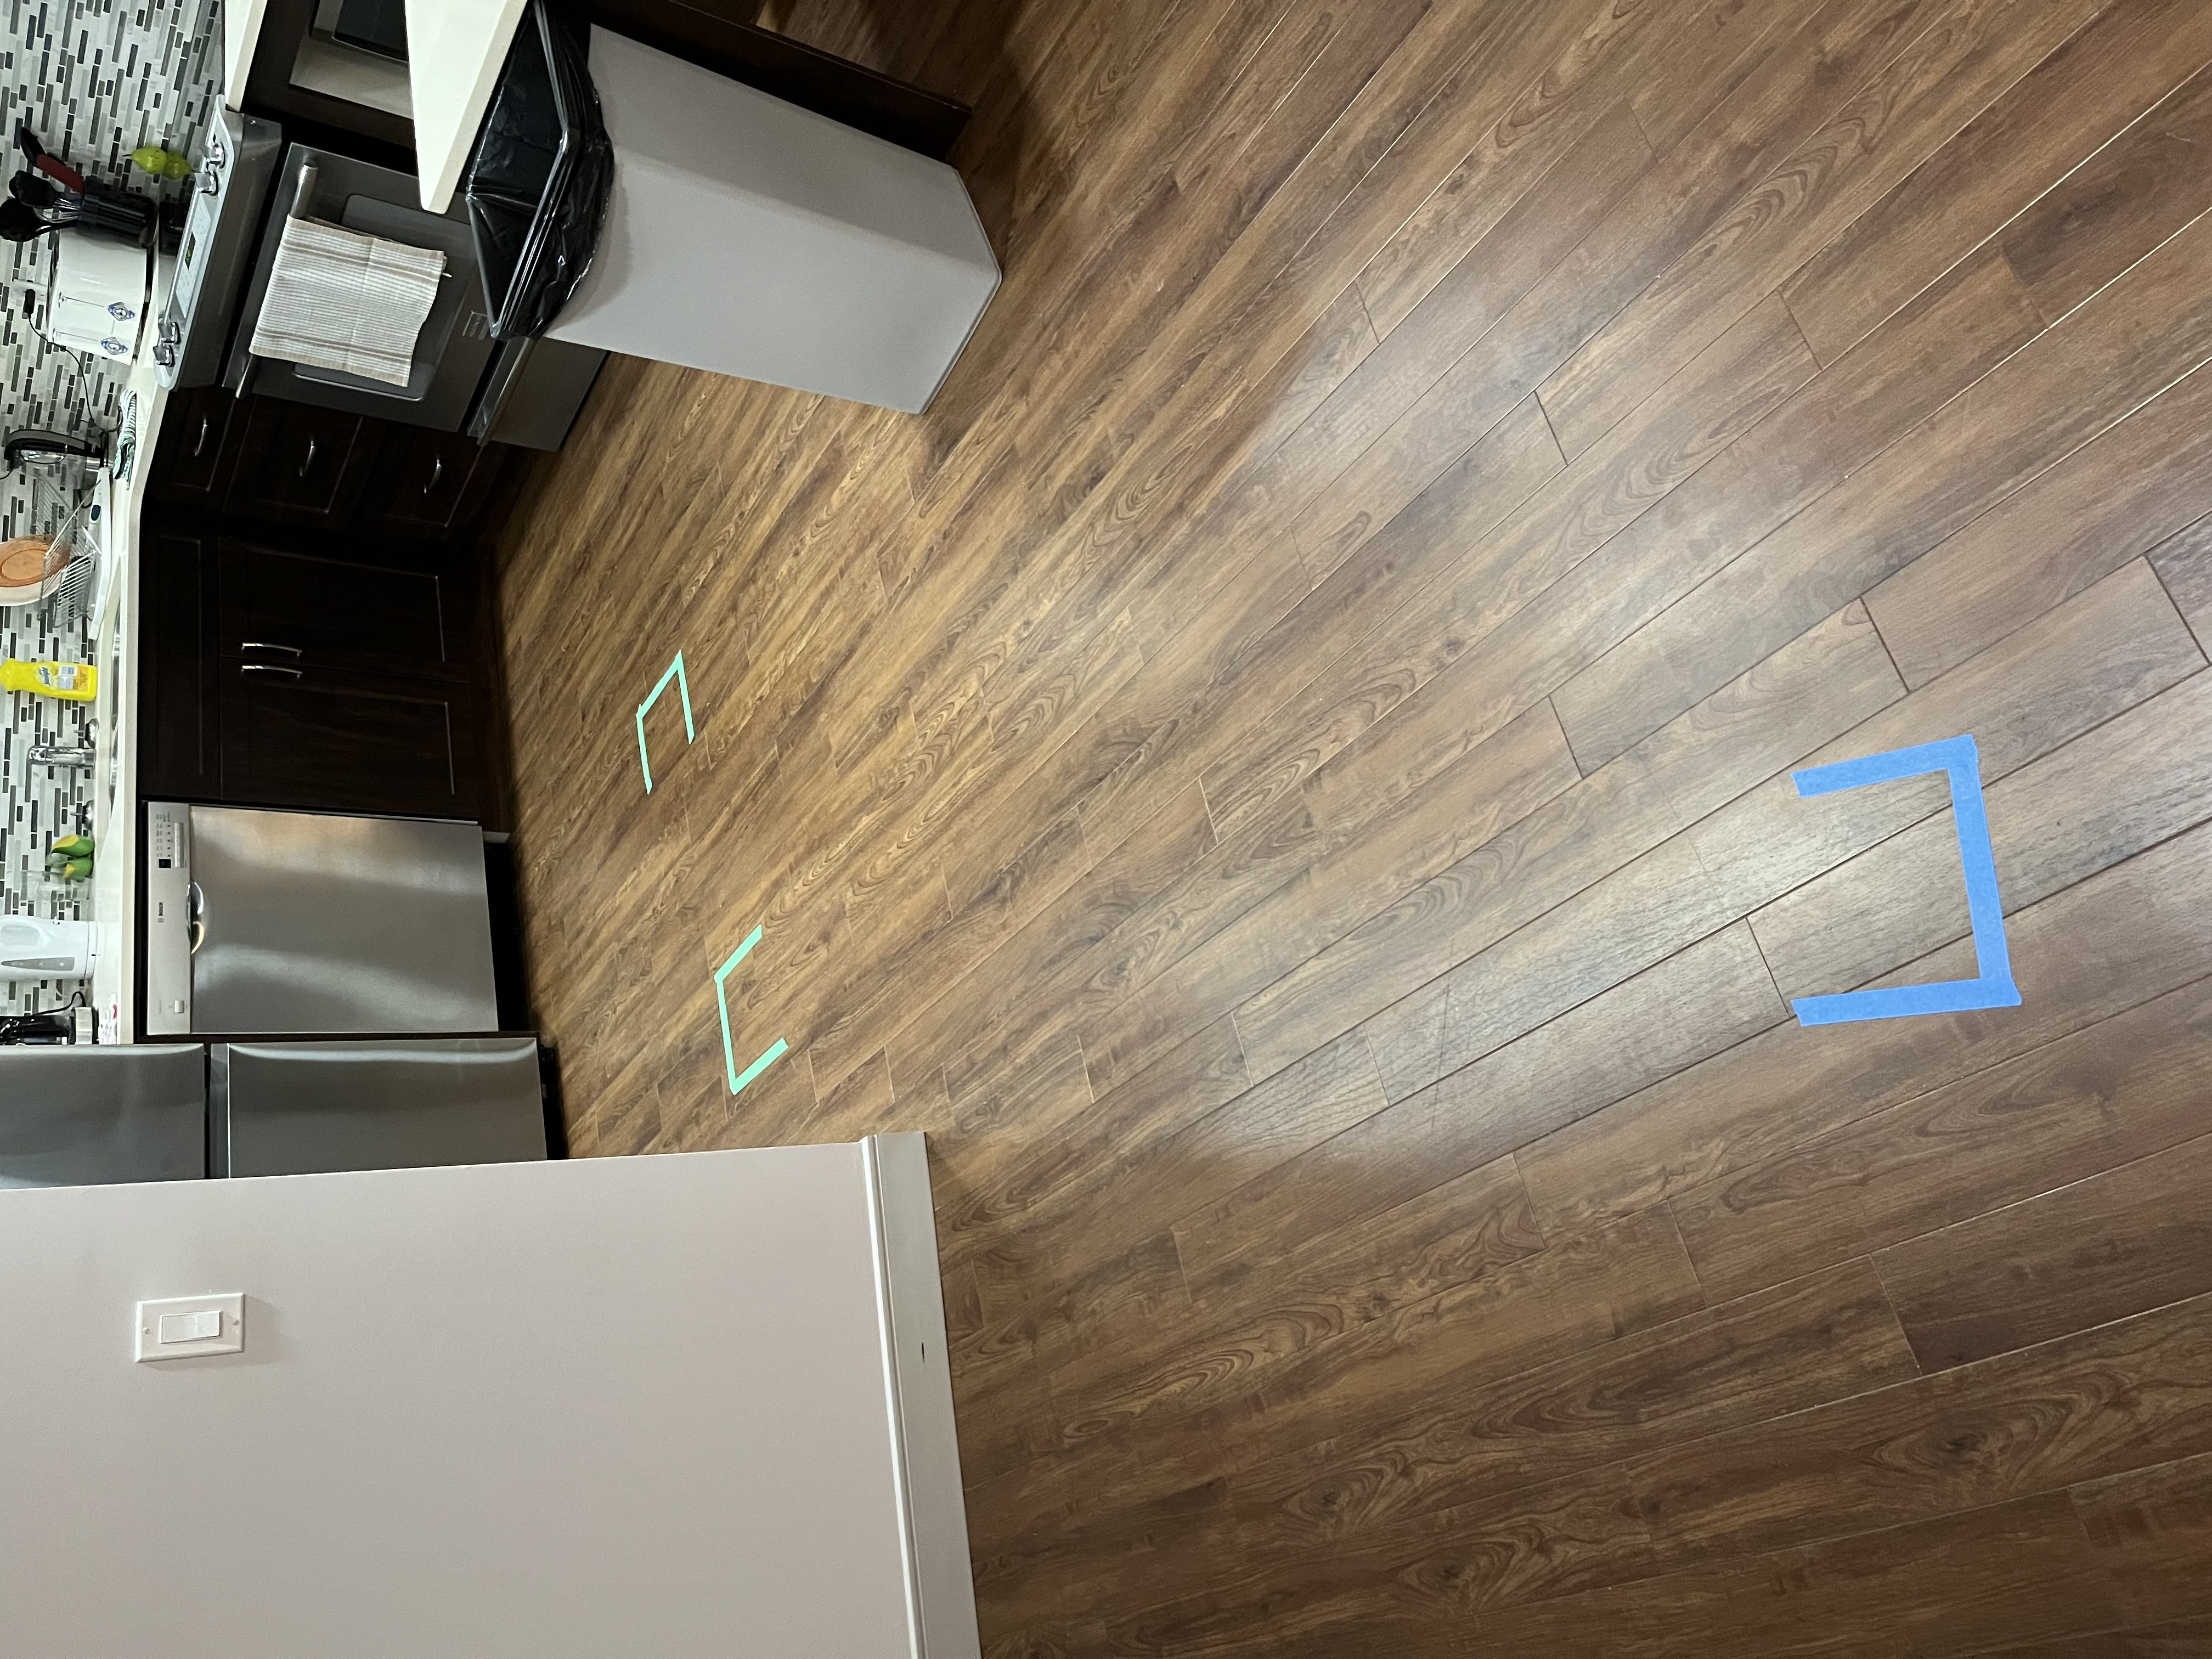
\includegraphics[width=0.6\textwidth, angle=-90]{tape.jpg}
    \caption{Box tape placement at the stove, fridge, and dining table. Participant's toes 
    and sides of feet should touch the tape.}
    \label{fig:tape}
\end{figure}

Following the tape placement guidelines outlined at the beginning of this section,
tape was placed at or near the following locations. Refer to the AUTOCAD floor plan for 
the location of the rooms (Figure \ref{fig:floorplan}):
\begin{itemize}
    \item The Hallway between Living Room and Kitchen facing the Dining Table.
    \item The Living Room facing the Desk.
    \item The Bedroom facing the bed.
    \item The Hallway between the bedroom and the bathroom, facing away from the wall.
    \item Bathroom facing the toilet.
    \item Kitchen facing the stove.
\end{itemize}

\begin{figure}[ht]
    \centering
    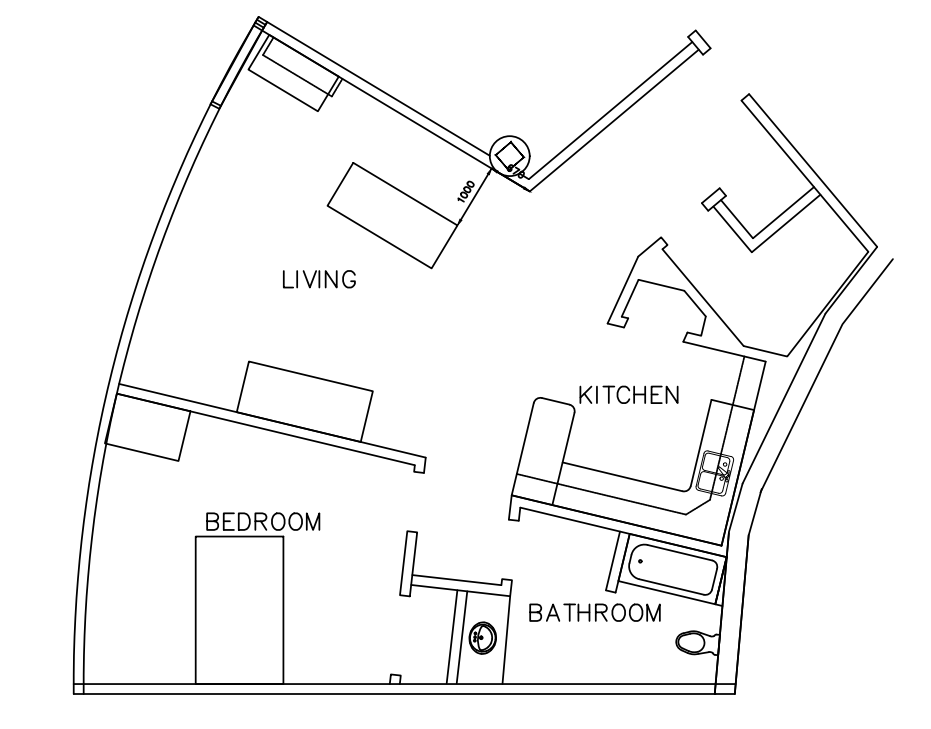
\includegraphics[width=0.8\textwidth]{floorplan}
    \caption{Floor plan of the ILS. Positions where the participant stood 1 meter
    from appliances or furniture are marked in the green "open" box on the floorplan.
    }
    \label{fig:floorplan}
\end{figure}

\clearpage
\subsection{Protocol}
A stopwatch python script was created with predetermined labels and used as the ground truth 
for positions. A single participant wore the tag on a 3D printed necklace mount (Figure \ref{fig:necklace}). 
The measuring tape was used to measure the height from the ground and height when squatting.
For this participant, the standing height was \textbf{144cm} and the squatting height was \textbf{68.5cm}.

\begin{figure}[ht]
    \centering
    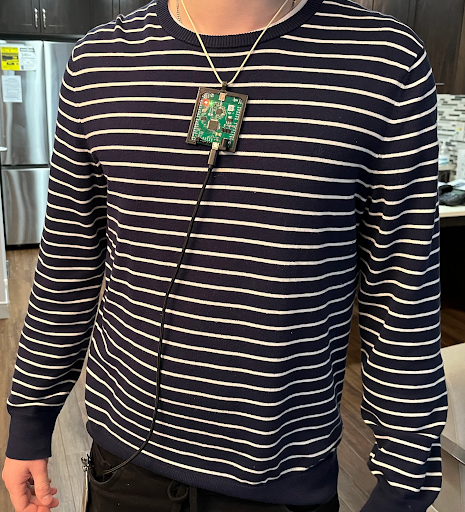
\includegraphics[width=0.7\textwidth]{necklace}
    \caption{The Pozyx tag mounted in a custom 3D printed necklace mount.}
    \label{fig:necklace}
\end{figure}

The protocol had the following steps:
\begin{enumerate}
    \item At the first location (Hallway Between Living Room and Kitchen) stand still for 10 seconds
    \item Squatt still for 10 seconds.
    \item Move to next position.
    \item Repeat steps 1-3 until all of the positions have been reached.
    \item Finally return to the first position (Hallway Between Living Room and Kitchen)
\end{enumerate}

There were 3 trials for each configuration. Following the guidelines from 
the Pozyx Creator Setup \cite{noauthor_configuration_nodate} anchors were 
staggered at heights of 1.4m and 2.4m (ceiling height) for 4, 5, 6, 8, and 10 anchors.
A configuration where anchors were all low (10cm) were tested for 8 anchors and configurations
where anchors were all high (2.4m) were tested for 8 and 9 anchors.

\section{Results}
Trials for each configuration were aggregated, transition periods were removed, 
data of interest was time normalized and the error and standard deviation of each
location while standing and squatting were calculated. An as-built AUTOCAD file of the 
ILS was used to obtain the real position and used in the calculation of the error 
between measured versus the actual position. The results of the experiment are summarized
in the heatmap tables (Figures \ref{fig:xposstats}, \ref{fig:yposstats} and \ref{fig:zposstats}) 
with a minimum darkness set at 30cm and a maximum darkness set at 60cm.

\begin{figure}[ht]
    \centering
    \begin{subfigure}[b]{\textwidth}
        \centering
        \includegraphics*[width=\textwidth]{x_errors}
        \caption{}
    \end{subfigure}
    \begin{subfigure}[b]{\textwidth}
        \centering
        \includegraphics*[width=\textwidth]{x_stds}
        \caption{}
    \end{subfigure}
    \caption{The positional error in X (a) and the standard deviation in X (b) at each location
    and body position
    }
    \label{fig:xposstats}
\end{figure}

\begin{figure}[ht]
    \centering
    \begin{subfigure}[b]{\textwidth}
        \centering
        \includegraphics*[width=\textwidth]{y_errors}
        \caption{}
    \end{subfigure}
    \begin{subfigure}[b]{\textwidth}
        \centering
        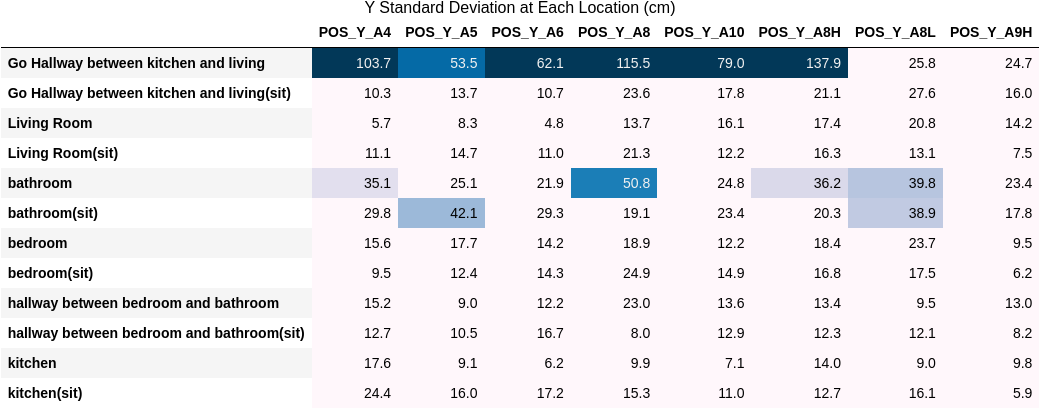
\includegraphics[width=\textwidth]{y_stds}
        \caption{}
    \end{subfigure}
    \caption{The positional error in Y (a) and the standard deviation in Y (b) at each location
    and body position}
    \label{fig:yposstats}
\end{figure}

\begin{figure}[ht]
    \centering
    \begin{subfigure}[b]{\textwidth}
        \centering
        \includegraphics*[width=\textwidth]{z_errors}
        \caption{}
    \end{subfigure}
    \begin{subfigure}[b]{\textwidth}
        \centering
        \includegraphics*[width=\textwidth]{z_stds}
        \caption{}
    \end{subfigure}
    \caption{The positional error in Z (a) and the standard deviation in Z (b) at each location
    and body position}
    \label{fig:zposstats}
\end{figure}

\clearpage
\section{Discussion}

\subsection{X Position}
Visually, the heatmap of error in the X position shows different spots 
where the system struggled to obtain the location based on the AUTOCAD as-builts 
depending on the configuration selected.
For 4, 5 and 6 anchors, the errors seemed to be larger in the living room
and the hallway between the kitchen and the living room. 8, 10, 8 (L)ow, 8 (H)igh, and 9H
anchors seemed to struggle most around the bathroom and bedroom area. 
The standard deviation in X position seems to follow a similar pattern where 
4, 5 and 6 anchors have higher standard deviation in hallway between the kitchen and living
area and 8, 10, 8 (L)ow, 8 (H)igh, and 9H seems to struggle the most in the bathroom.
Out of all of the configurations the 9H configuration has the most locations
where the standard deviation is acceptable.

\subsection{Y Position}
For 4, 5, and 6 anchors, the error seems to increase in the seated position
meaning that there may be some dependence on the Z position. This occurs 
in the hallway between the kitchen and the living room, the bathroom and the 
hallway between the bedroom and bathroom.
There seems to be a large struggle for 8, 10 and 8H anchors to pinpoint the Y
position in the hallway between the kitchen and the living, the living room
and the bathroom. The 8L anchor configuration struggled when the in the bedroom,
but was overall within or near the acceptable threshold of 30cm. 9H anchors
overall seemed to be the best at determining the Y position with mild 
errors at the hallway between the kitchen and the living room, the living room 
and the bathroom.

In terms of standard deviation, anchor configurations 4, 5, 6, 8, 8H, and 10 
had trouble at a height of 144cm, but otherwise had low standard deviation.
8L had minor issues regarding standard deviation in the bathroom 
but was otherwise low. The 9H configuration seemed to yield
the lowest standard deviations in the Y Position. 

\subsection{Z Position}
The Z position at many of the locations and all configurations seem 
to deviate from the measured heights and have high error. 
Only the 8H and 9H configurations have acceptable standard deviations
for most of the rooms (there is still some struggle in the bathroom).
Considering the inaccuracies in the Z positioning, it is recommended
that the Z not be used as a absolute source of truth for height. 
Rather Z position should be used relative to another reference tag 
with the 9H configuration. For example, a necklace tag may be combined
a wrist tag. When standing, the position of the wrist may be compared 
with the position of the necklace to determine if the wrist is 
above, below or at chest height.

\subsection{Overall}
The 9H configuration seems to provide the most reliable data when observing
the standard deviations of the X, Y, and Z positions. With this configuration,
each room had around 4 anchors surrounding it Figure \ref{fig:anchorplacement}

\begin{figure}[ht]
    \centering
    \includegraphics*[width=0.8\textwidth]{floorplananchors}
    \caption{ILS Floorplan with the 9 anchors all high.}
    \label{fig:anchorplacement}
\end{figure}

Though the inaccuracies in the hallway, living room, bathroom and bedroom may
prevent the 9H configuration from using heuristics for classification at these 
locations, the inherent repeatability evident in the low standard deviation in 
each axes of the position can make the position data from the 9H configuration
a candidate for machine-learning based classification. 
% ----------------------------------------------------------------------------------------------------
